\subsection{Afstandssensorer}

\begin{figure}[H]
\centering
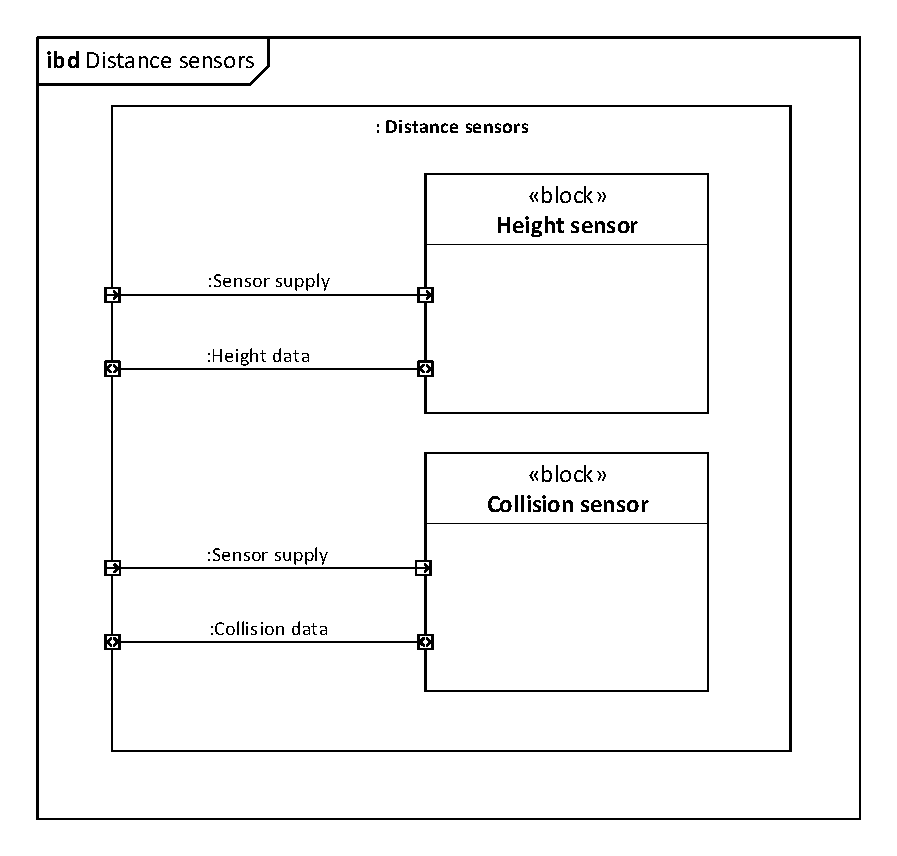
\includegraphics[width=1\textwidth]{Billeder/IBD/ibd4_distancesensor.pdf}
\caption{ibd - distance sensor}
\label{fig:ibd_distancesensor}
\end{figure}

\begin{table}[H]
	\centering
		\begin{tabular}{|p{2.5 cm}|p{5.5 cm}|p{2.5 cm}|p{2.5 cm}|} 
		\hline
			\textbf{Signal navn} 	& \textbf{Signal beskrivelse}		& \textbf{Out} 				& \textbf{In}     \\ \hline
			Sensor supply & 5V DC.  & Arduino. & Height sensor.  \\ \hline
			Height data & RX / TX signal. & Arduino.	& Height sensor.	\\ \hline
			Sensor supply & 5V DC. & Arduino. & Collision sensor.	\\ \hline
			Collision data & RX /TX signal & Arduino. & Collision sensor.			    \\ \hline  
		\end{tabular}
	\caption{Forbindelser til: \textbf{ibd} Distance sensor}
	\label{tab:IBDDistancesensor}
\end{table}
